\documentclass[11pt]{wlscirep}
\usepackage[utf8]{inputenc}
\usepackage[T1]{fontenc}
\usepackage{gensymb}
\usepackage{amsmath}

\title{Hydroclimate variability structures social interaction in the prehistoric American Southwest}

\author[1,*]{Nicolas Gauthier}

\affil[1]{School of Human Evolution and Social Change, 900 S Caddy Mall, Tempe, USA}

\affil[*]{Nicolas.Gauthier@asu.edu}

\keywords{Archaeological Networks, Spatial interaction model, Drought}

\begin{abstract}
  Do small-scale farmers prefer to interact with others experiencing different weather patterns? In agricultural societies, farmers' social networks help absorb the impacts of droughts and floods by facilitating resource flows to affected settlements and population flows away from them. This property of social networks depends on the degree to which the network connects populations in topographically accessible locations that tend to experience different weather patterns. The patterns by which droughts covary in space and time thus ought to interact with patterns of landscape connectivity to structure prehistoric social networks. Here I analyze a set of 7.5 million artifacts collected from nearly 500 archaeological sites in the precontact American Southwest, and estimate how the flow of social information between sites varied as a function of distance and growing-season aridity. I find that although the intensity of social interaction in the past was highly distance dependent, interactions between regions experiencing different domains of externally-forced drought variability (e.g. Pacific vs Atlantic) is higher than would be expected by distance alone. These findings add empirical detail to ideas long theorized in anthropology, emphasizing the need for more precise definitions of ``climate'' in studies of human-environment interaction, and will be key for forecasting potential social responses to drought events in the developing world of today.
 \end{abstract}

\begin{document}

\flushbottom
\maketitle


\thispagestyle{empty}


\section*{Introduction}
Human populations in dryland environments rely on suites of social and physical infrastructure to manage environmental risk. Food storage is one effective strategy for preserving bulk grains in dry environments, and storage features are common in the ethnographic and archaeological records \cite{Spielmann2011SustainableEnvironments}. Irrigation is another effective strategy, redistributing soil moisture in space and time to create microenvironments suitable for agriculture. But a reliance on physical infrastructure shifts farmers' vulnerabilities from droughts to floods, and would have demanded significant labor investments to monitor and maintain \cite{Dominguez2005}. Such strategies would have been effective for managing small-scale variability (year-to-year and field-to-field), but would have been vulnerable to long-lasting, spatially extensive droughts or pluvials \cite{Halstead1989}. In years of drought and famine when food stores are low, farmers often rely on their social networks to transport food and other resources to affected settlements or move people away from them, depending on the scale and severity of the event. In either case, information is the central currency of the network. A more general approach to these systems views them as a form of social infrastructure \cite{STRAWHACKER2015}, channeling the flow of energy between spatially structured populations in much the same way as food webs channel energy in ecosystems \cite{Crabtree2015,Crabtree2017ReconstructingStates}. The importance of exchange networks as mechanisms of risk reduction is a common qualitative observation in the ethnographic and archaeological records (TODO cite). This study adds an empirical dimension to this discussion using a long-term archaeological case study.%(scudder1962, cashdan 2001, waddel 1975, colson 1979, speilmann 1982, 1986, cashdan 1985, wiessner 1982, werner 1983, yengoyan 1972, duff 1998, 2002, cameron 1995, jaskoff and adams 1977, crumly 1979 TODO cite)

Recent theoretical and empirical work has begun to address how spatial, social, and environmental factors structure exchange networks \cite{Nolin2010Food-SharingIndonesia,Koster2014,Hao2015,Schnegg2015}. There is an unavoidable trade-off between the costs and benefits of maintaining infrastructure. The desire to gain those benefits while avoiding the costs tempts free-riders who take more than their fair share. Risk sharing networks can effectively pool and mitigate the risk of drought, but they are sensitive to the costs of information transfer. If each individual's resources are not common knowledge, it becomes difficult to monitor and sanction free riders \cite{Hao2015a}. Face to face social interaction is critical for monitoring and sanctioning free riders (TODO cite ostrom here with face to face interaction and free riders). Face-to-face interaction is the source of all other social processes, such as trade, marriage, copying (TODO cite scaling folks?). Freeriding can lead to the breakdown in this critical social infrastructure when it is most needed (TODO cite kohler and van west 1996). More restricted sharing rules can be effective \cite{Hegmon1996}, but can also be sensitive to the asymmetric accrual of debts if one party's food supply is more volatile than the other's \cite{Crabtree2015}. Similar information constraints influence migration networks. Imperfect information about conditions in potential target locations may mean individuals will make costly trips that serve no benefit, or fail to make trips when it is in their clear interest to do so \cite{Anderies2011a}. Distance ultimately constrains the flow of information on these networks, as the further one must travel to interact with a social partner the greater will be the cost in time, money, and energy. Anthropological theory predicts (TODO REfs) that the benefits of interaction between areas with different rainfall patterns will often outweigh the costs of distance, and that norms and institutions encouraging such long distance ties are likely to evolve. Thus, exchange is not independent of the environment, as the specific biophysical contexts of exchange systems structures the potential costs and benefits of interaction.

A central principle in archaeology is that the spatial and temporal patterns of environmental variability can be used to predict ideal cultural responses, and these expected cultural responses can be compared to archaeological observations to test the importance of that particular pattern of environmental variability \cite{halstead1989}. This process yields empirical predictions testable in the archaeological record. Archaeology, with its focus on the material correlates of human behavior over long time spans, is uniquely suited to address how social and physical infrastructure modulates human interactions with the environment. Not only do archaeologists catalogue the remains of field systems, road networks, canals, and other components of hard infrastructure directly, but also the ceramics, raw materials, and luxury goods that are the material correlates of past networks of exchange and interaction. This approach, while valuable, is sensitive to how exactly one defines ``climate variability.'' Droughts in the American Southwest, for example, have multiple dynamic origins. Winter rainfall is delivered by large-scale precipitation and mesoscale storms brought by westerly winds, and summer precipitation falls from convective storms associated with southerly Monsoonal winds. Rainfall in both seasons varies markedly year-to-year and, because the majority of annual precipitation can fall in only a handful of storms, is highly unpredictable in space. Drought conditions are usually initiated by global ocean-atmosphere \textit{teleconnections} such as unusually cool Pacific sea surface temperatures associated with the La Ni\~{n}a phase of the El Ni\~{n}o-Southern Oscillation (ENSO), but the length of these dry spells often reflects more localized positive feedbacks between vegetation and soil moisture \cite{Koster2004RegionsPrecipitation,Ault2014AssessingData}. Which of these sources of variability matter most to the prehistoric farmers who once lived there? The central contribution of this study is a more rigorous empirical assessment of climate variability than is common in previous work.

Droughts are complex biophysical phenomena. Precipitation, temperature, radiation, humidity, wind speed, ground water, vegetation all contribute to a region's average \textit{climatic water balance}, the difference between precipitation and potential evapotranspiration. Feedbacks between these variables drive variability on multiple spatial and temporal scales. It is useful to distinguish between three nested types of droughts based on their scale and severity, in increasing order of time scale. Meteorological droughts are any short-term dry spell. Agricultural droughts last a year or more, depleting soil moisture and killing crops. A hydrological drought can last from several years to decades, as progressive losses of vegetation and groundwater lock in arid conditions. These are events such as the Dust Bowl of the last century, as well as the extensive ``megadroughts'' observed in the proxy record of North America. These events can arise naturally from the internal variability of the world's ocean and atmosphere, but can also be triggered by volcanic eruption and other external events. Hydrological droughts are most likely to require buffering via exchange networks, because farmers can mitigate one-year agricultural droughts storing a proportion of each year’s harvest.

Here I use an empirical archaeological case study to examine the relationship between drought variability and human social networks over the long term. The North American Southwest is extensively studied both in archaeology and climate science. Rates of archaeological site preservation and recovery are exceptionally high in this region. Nearly two centuries of survey and excavation have yielded extensive, high quality settlement pattern data. Detailed inventories of material culture at hundreds of archaeological sites provide an unparalleled view of the structure and dynamics of past social networks. The climate of this period over the last 2,000 years has been intensively studied by paleoclimatologists and climate modelers, and is recorded in a strong tree ring archive. I use principal components analysis (PCA) to extract latent patterns of spatial and temporal drought variability. PCA is a common tool for extracting modes of variability in the climate sciences, but has been used only rarely in comparison to archaeological data \cite{Weiss1982,vanwest}. Furthermore, even if climate variability plays an important role in social network formation, network data representing flows of information and people have several endogenous characteristics that must be correctly modeled in order to make accurate statistical inferences. Spatial interaction models and their variants are used extensively across the social and natural sciences (TODO cite). Although spatial interaction models are seeing increasing use in archaeology as tools for dynamical simulation (cite wilson, bevan et al, rivers evans), their use as a statistical model received unequal attention (Tobler, Johnson, hodder) due to the difficulty in gaining empirical estimates of interaction strength. Our approach, combining PCA analysis of climate variability with statistical spatial interaction models, is the first of its kind in archaeology. This work opens the door for a more rigorous evaluation of dynamical theories against the empirical archaeological record and integration of climate and society as dynamical systems.

%the flow of social information along exchange networks.

\section*{Results}

\subsection*{Six modes of variability explain 80\% of drought in the Southwest}
I extracted robust spatio-temporal modes of drought and pluvial variability from a 100 year observational record of the Standardized Precipitation-Evapotranspiration Index (SPEI), a drought index that measures the deviation from average climate water balance for a given month on varying time scales. SPEI values are interpretable as z-scores in a normal distribution (i.e. a value of 1 is one standard deviation wetter than average for that location, -1 is one standard deviation drier). As hydrological droughts during the summer growing season are most likely to influence exchange networks, I focused on the 24-month SPEI calculated in the August of each year. I used a PCA to decompose the 100 years of space-time drought data into leading modes of variability (TODO define). The principal components (PCs) represent SPEI time series that are maximally representative of the entire data set, and the leading 6 PC time series together explain 83\% of the SPEI variance from the 100 year observational record. 

To reveal the latent spatial structures associated with the temporal modes of variability, I map the spatial patterns associated with each of the leading 6 PCs (Figure \ref{fig:reofs}). PCs beyond the leading 6 were not retained, as they represent spatially and temporally incoherent variability and spurious correlations introduced by sampling error in the observational record. We rotated the 6 PCs before mapping, in order to capture more physically meaningful patterns and minimize statistical artifacts. The results are robust, recurring patterns of spatially-coherent variability, and can be interpreted as the degree to which 100 year record at each grid cell correlates with the associated rotated PC time series. The spatial and temporal patterns associated with the leading 6 PCs allows us to trace the sources of each mode of variability back to the global climate system.

%\begin{figure}[!htbp]
%\centering
%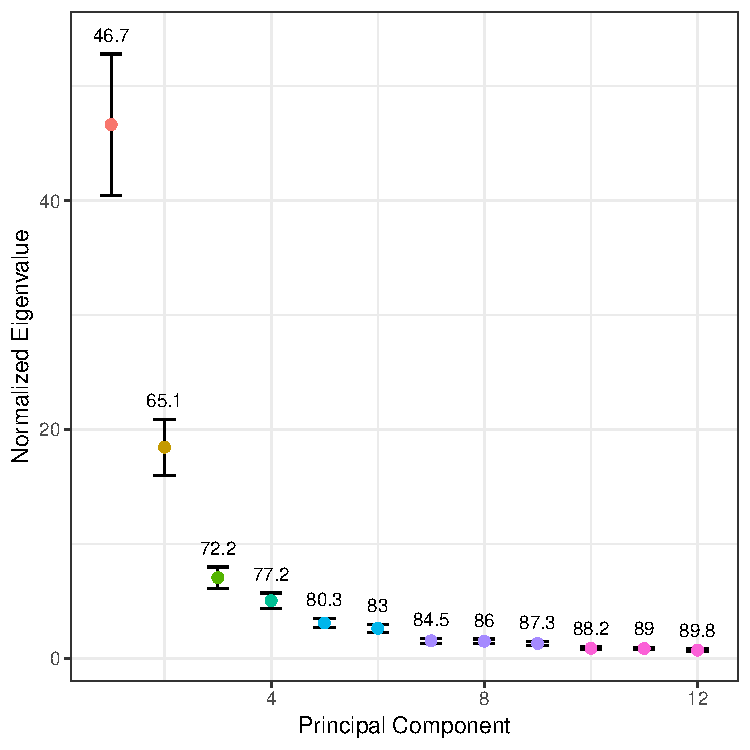
\includegraphics[width=.5\linewidth]{figures/variance_explained.pdf}
%\caption{Scree plot of the leading 12 PCs and their associated eigenvalues. The PCs are arranged in order of decreasing percent variance explained. Standard errors for the eigenvalues are calculated using North's rule of thumb, and sets of eigenvalues with poorly-separated errors are colored the same.}
%\label{fig:scree}
%\end{figure}

\subsection*{Pacific and Atlantic influences predominate, with complex topographic interactions}

Drought variability in the American Southwest is primarily influenced by tropical Pacific sea surface temperatures, additional complex interactions with the North Pacific and Atlantic. The regional expression of these global influences is in turn mediated by local terrain and atmospheric circulation. These same patterns from the observational period also show up in reconstructions pulling in data from 1100 CE to present. This underlies the fact that these are robust, time invariant spatial modes. The correlation between the amplitude time series for matching spatial patterns was XXX. These spatial and temporal drought patterns, and their hypothesized forcings from the global climate system, are largely consistent with those from other studies using varied observational data and time windows (cook meko et al 1999 j climate, mccabe et al 2004, mccabe and dettinger 1999, dean et al,hermann et al 2016, ryu svoboda 2010, seager hoerling 2014!<- really good, comrie and glenn 1999)\footnote{For simplicity I refer to these as modes of ``drought'' variability, but emphasize that the SPEI measure captures the full spectrum of moisture variability, from extreme drought and pluvial events to finer variability in moisture and aridity. The key point is that all this variability maps onto similar spatial modes, due to their reliance on the same underlying atmospheric dynamics.}.

\begin{figure}[!htbp]
\centering
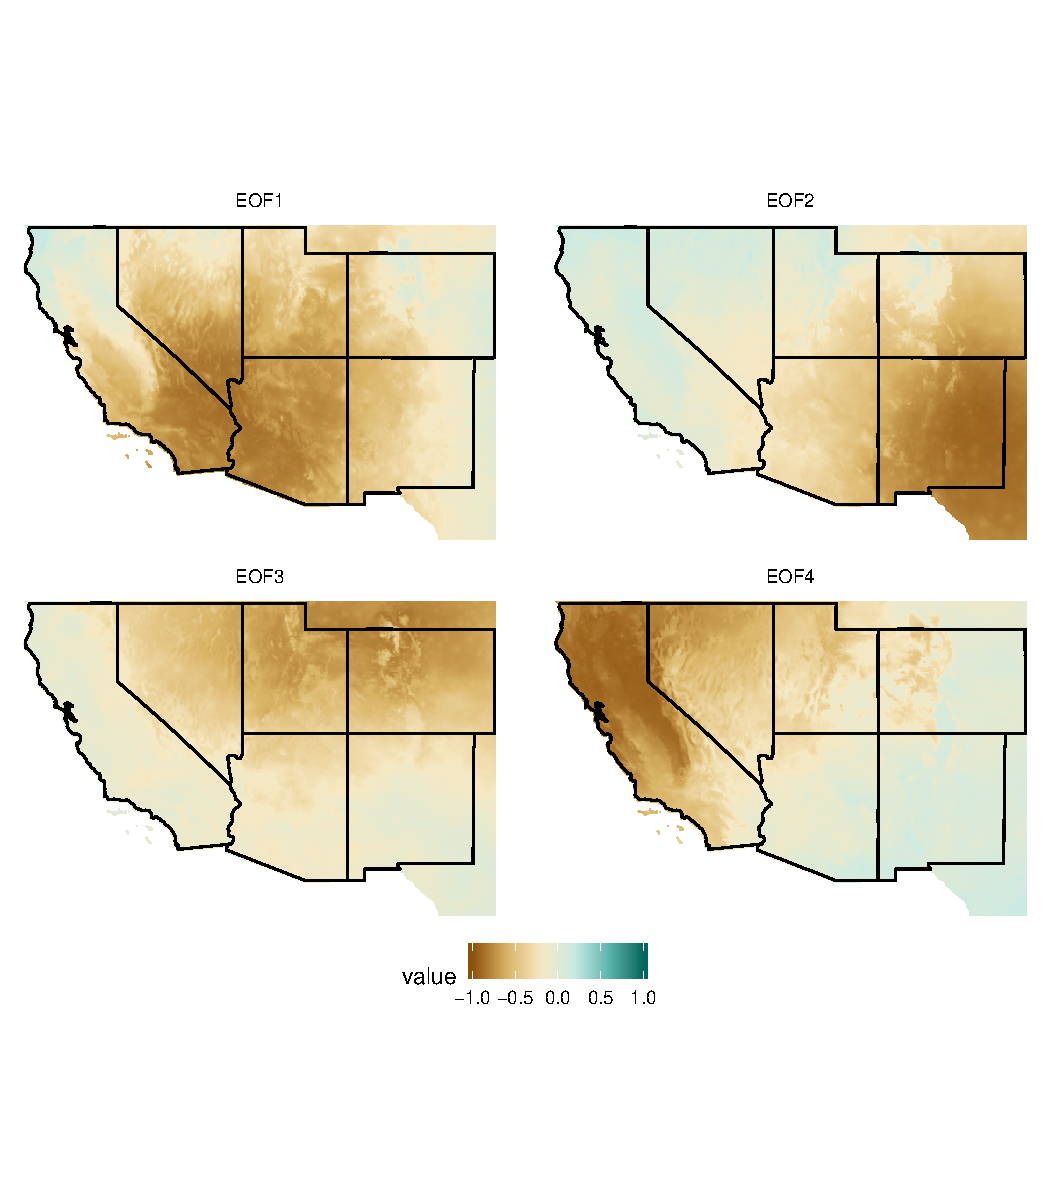
\includegraphics[width=.8\linewidth]{figures/reof_observed.pdf}
\caption{Leading 6 rotated empirical orthogonal functions. The empirical orthogonal functions are the spatial patterns associated with their respective principal component time series. The REOFs are the eigenvectors of the space-time covariance matrix, and the PCs are the eigenvalues. The leading six EOFs, which together explain 77\% of interannual drought variability in the observational record, were then subjected to varimax rotation, to make the spatial patterns more physically meaningful by relaxing the spatial orthogonality constraint.}
\label{fig:reofs}
\end{figure}

PC1 represents a center of action in the desert Southwest portions of California and Arizona, extending up to the northeast. It represents the influence of tropical Pacific sea surface temperatures, such as the North American Monsoon and tropical storms. This pattern is produced by southwesterly flow from the tropical pacific, bringing moisture up across the low desert zones. The pattern attenuates with gains in elevation, as distance from the ocean increases. On a global scale, this pattern is associated with a mode of Atlantic sea surface temperature variability called the Atlantic Multidecadal Oscillation. PC2 similarly represents southeasterly flow from the Gulf of Mexico, with a center of action in eastern New Mexico. As with PC1, the pattern attenuates with increasing elevation and distance from the ocean, due to orographic and continentality effects, respectively. It represents cyclonic storms coming from the Gulf of Mexico, in turn influenced by variability in Atlantic sea surface temperatures. The pair of Pacific and Atlantic SST dominated drought patterns in the Southwest has been previously hypothesized before in the context of archaeological change (dean and van west), but the level of spatial detail here far surpasses previous studies. There in the context of a ``bi-modal precipitation distribution'', meaning the distinguishing between regions with both summer and winter dominate precipitation (PC1) and those with just summer dominate precipitation (PC2). Although specifically growing season (summer) variability is measured here, the pattern is also consistent with winter moisture variability, as the 24 month SPEI index integrates the long lag effects of winter moisture, and the summer and winter patterns are governed by similar atmospheric teleconnections to Pacific SST variability. The strength of the summer monsoon has a strong soil moisture memory effect, and is influenced by the preceding winter's precipitation.

Land falling Pacific storms. Separation between Pacific and Gulf of Mexico influences. Meet along the rocky mountains, exactly where is determined by pressure systems. (Liu et al 2010)

These patterns reflect a combination of advection of moisture from the Pacific or gulf of mexico, and the orientation and height of the mountains.
Associated with different zones of moisture transport (Liue et al 2010)

so EOF 5 and 6 are arctic and continental influences, respectively

hu and feng support interpretation that reof 1 and 2 are different monsoon regimes, influenced by topography and moisture sources.
PC2 is the 1950s drought (cote fye stahle cook)

PC3 is a round region corresponding with the Colorado Plateau. The mode of variability here is likely temperature dependent, reflecting interactions with radiation at increased elevation. The pattern covaries with elevation, but they are not exact (TODO R2 = ). Variability here is likely linked to Atlantic multidecadal variability. Perhaps the 4 corners high.

PC4 clearly represents the influence of westerly flow off the Pacific Ocean, and the orographic effect of the Sierra Nevada mountains intercepting this flow. These include atmospheric rivers (TODO cite uh that paper), and are associated with coastal droughts in California. PCs 5 and 6 both represent centers of action far removed form the study area. PC5 is centered over the great plains and attenuates across the Rocky Mountains. PC6 is centered in the North West. Both these patterns are much less salient in the US Southwest, so Iexpect them to impose less of a structure on social dynamics in the Arizona-New Mexico study area.

% emphasize that different oceans influence different patterhsn. the question of teleconnections is a wider one because they correlate and are nesetd on different scales. amo and pdo both influece el nino, for example.  Hense why the spatial patterns stay moslty the same as you change the spei time scale, but the pcs do change. 

\begin{figure}[!ht]
\centering
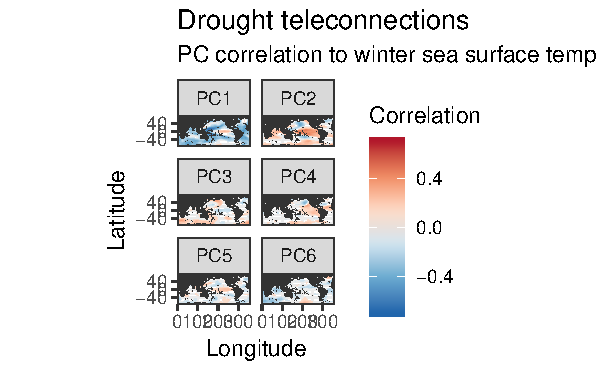
\includegraphics[width=.8\linewidth]{figures/sst_correlation.pdf}
\caption{Correlation between each observed PC amplitudes and winter sea surface temperature observations. PC1 is associated with el nino, pc2 with pdo, pc4 the blob, pc6 maybe NAO.}
\label{fig:sst-correlation}
\end{figure}

% temporal reconstruction

\begin{figure}[!ht]
\centering
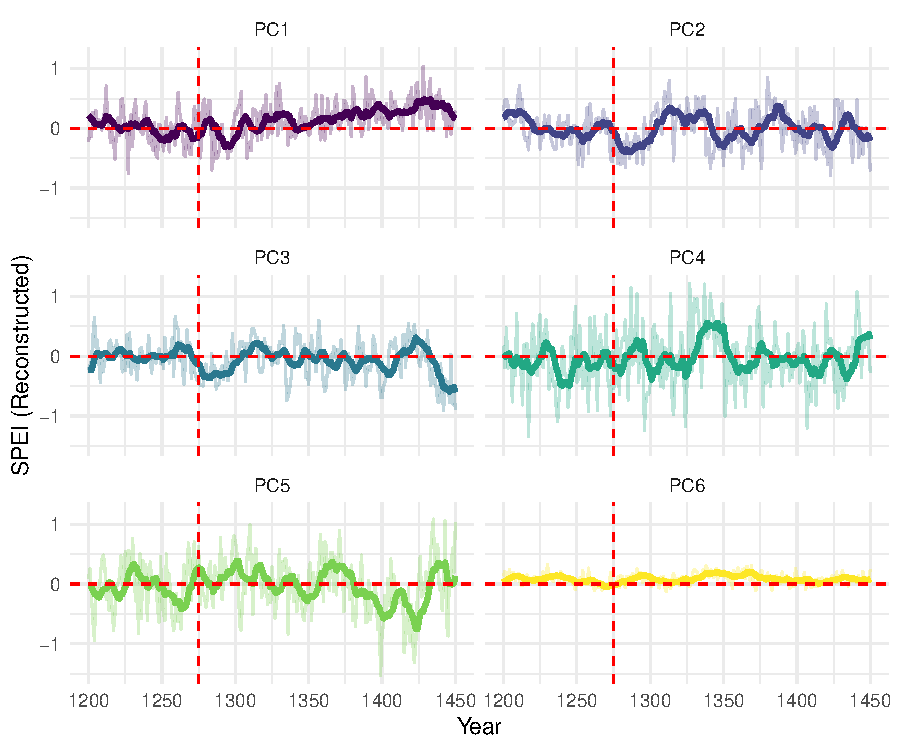
\includegraphics[width=.8\linewidth]{figures/spei_reconstruction.pdf}
\caption{}
\label{fig:spei-reconstruction}
\end{figure}


\begin{figure}[!ht]
\centering
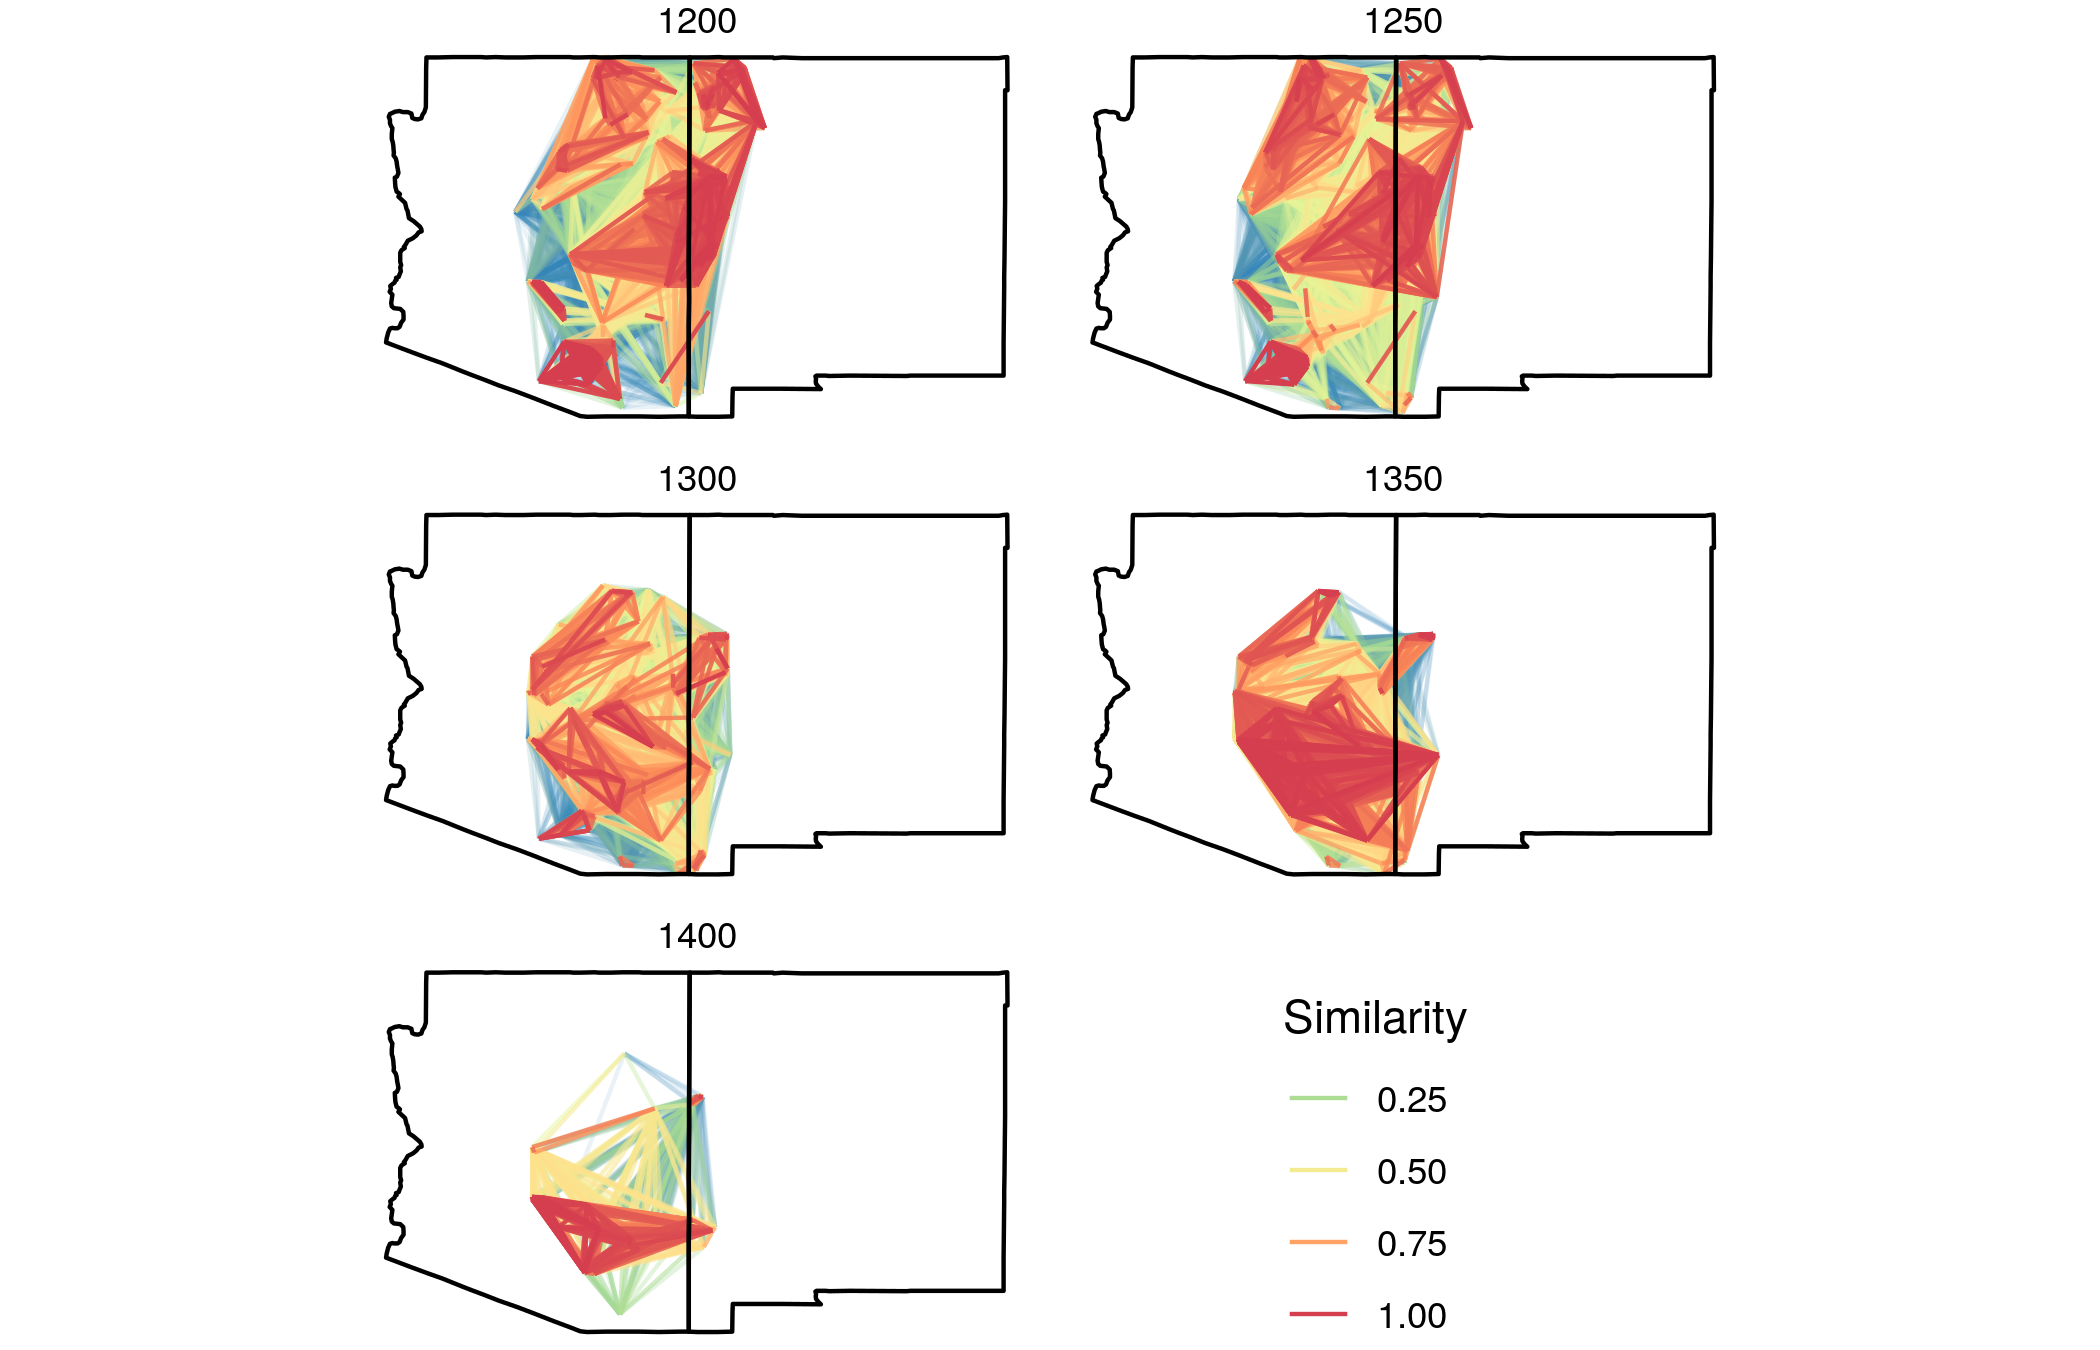
\includegraphics[width=.8\linewidth]{figures/similarity_network.png}
\caption{The \emph{Southwest Social Networks} dataset, version 1. Each line connects a pair of archaeological sites. Line color corresponds to the similarity of the artifact distributions between the pair. A similarity coefficient of 1 means that the sites share the exact same decorated ceramic wares in the exact same proportions, and a coefficient of 0 means there is no overlap in the ceramic assemblages. This similarity network can be interpreted as the degree of social interaction and cultural transmission between sites, whether via migration, trade, or copying. Networks are shown over successive 50 year time spans, starting at 1200 CE. A relatively stable network configuration starting at 1200 CE is interrupted by climatically-forced migrations near the end of the 1250 time step.}
\label{fig:network-plot}
\end{figure}

\subsection*{The intensity of social interaction decays with distance}
The null model for our statistical network analysis was that distance alone accounts for the intensity of social interaction. This model simply states that the longer the time it would take a traveller on foot to move between two locations, the greater the costs of social interaction. This concept is no different from isolation by distance or distance decay models in ecology and geography, but I refer to it as distance deterrence due to its role in decision making. I calculated the cost of moving between each pair of sites as the shortest amount of time it would take a traveler to move between them. I then used a nonlinear regression model to estimate the functional relationship between distance and interaction, as there is no agreed upon functional form in the social literature. 
The resulting \textit{distance deterrence function} (Figure \ref{fig:distance}) shows the estimated falloff in social interaction with increasing distance. The functional form of this distance decay closely resembles the Tanner function, a combination of the traditionally used exponential and power distance deterrence functions. This represents that multiple transmission processes, with different relationships to distance, are acting together to generate the variation in the archaeological record. The two main inflection points in the decay curve are both consistent with previous work in the ecology of human mobility. Their is a plateau effect distance plays no appreciable role in interaction between sites within a day's walk of one another (johnson but cites olsson 1965 and crumley 1979, ariadne). This suggests that distance only becomes a deterring factor dealing in multiday trips. The second inflection point, at roughly 10 days is consistent with estimates of area needed to sustain the minimum viable breeding population for human groups (are they consistent with the figures of 50km-80km from rautman and drennen and others? johnson finds no marriages past 60km, maize to chaco papers also have distance). This null hypothesis, that distance alone is sufficient to explain the observed divergences between archaeological assemblages, was sufficient to explain nearly 50\% of the variability in our dataset.  

Plateau of social interaction with communities who have daily face-to-face contact.

site hart 2016 for contrary and explain difference
%The Mogollon Rim acts as a severe bottleneck for spatial flows, with paths generally constrained to one of the three river systems, the Verde, Salt, and Gila, act to channel flow across this boundary.  

\begin{figure}[!htbp]
\centering
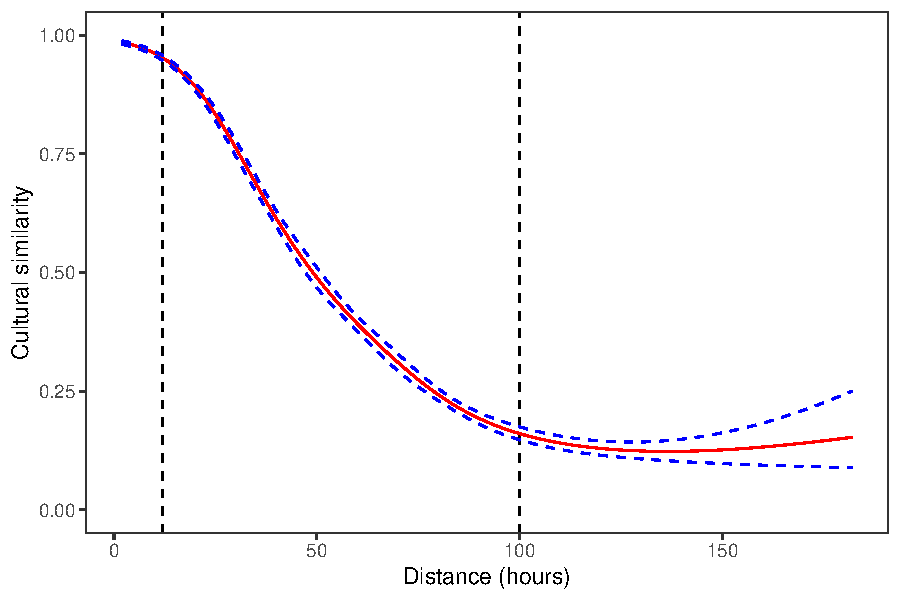
\includegraphics[width=.8\linewidth]{figures/distance_function.pdf}
\caption{Empirical distance deterrence function.}
\label{fig:distance}
\end{figure}

\subsection*{Drought variability explains a moderate but clear proportion of the intensity of social interaction}
A network model including the least-cost distance between sites with respect to each PC spatial pattern explains 57\% more of the variance in the network data than the distance-only null model. This increase in variance explained is small relative to the null model but is statistically clear. The model with drought variability also performs better than the null with respect to parsimony and goodness-of-fit, and has a consistently lower AIC and BIC than the null. As with the distance deterrence function, we have little \textit{a priori} assumptions about the functional form of these relationships. I thus used the same nonlinear regression approach, and used regularization techniques so that the algorithm will effectively select out irrelevant predictor variables. The resulting functional estimates show dependence on the particular drought pattern in question (Figure \ref{fig:smooths}). All functional forms reveal a close to pairwise linear structure, with no influence on social interaction between locations between 0.1 and 0.2 difference in drought pattern, reflecting the lack of significant distinction between opposing patterns at that scale. Beyond this threshold the relationships are roughly linear, but vary in sign and intensity. Sites that experience different patterns of monsoon variability (PC1 or eof3) are considerably more likely to interact than those by chance. Unexpectedly, the second clearest pattern is that sites are much less likely to interact across the PC 3 (eof6) pattern, suggesting that specific modes of variability can actually decrease the intensity of interaction, possible by encouraging conflict for resources. These results emphasize the importance of distinguishing different dynamic origins of drought variability, as different varieties of drought variability may have distinct influences on social interaction.


reof 1 is stongly positive flooding increasing after 1350, corresponding to floodingin the hohokam region, period of hihg variability in reof2. also correspods to salado culture

\begin{figure}[!htbp]
\centering
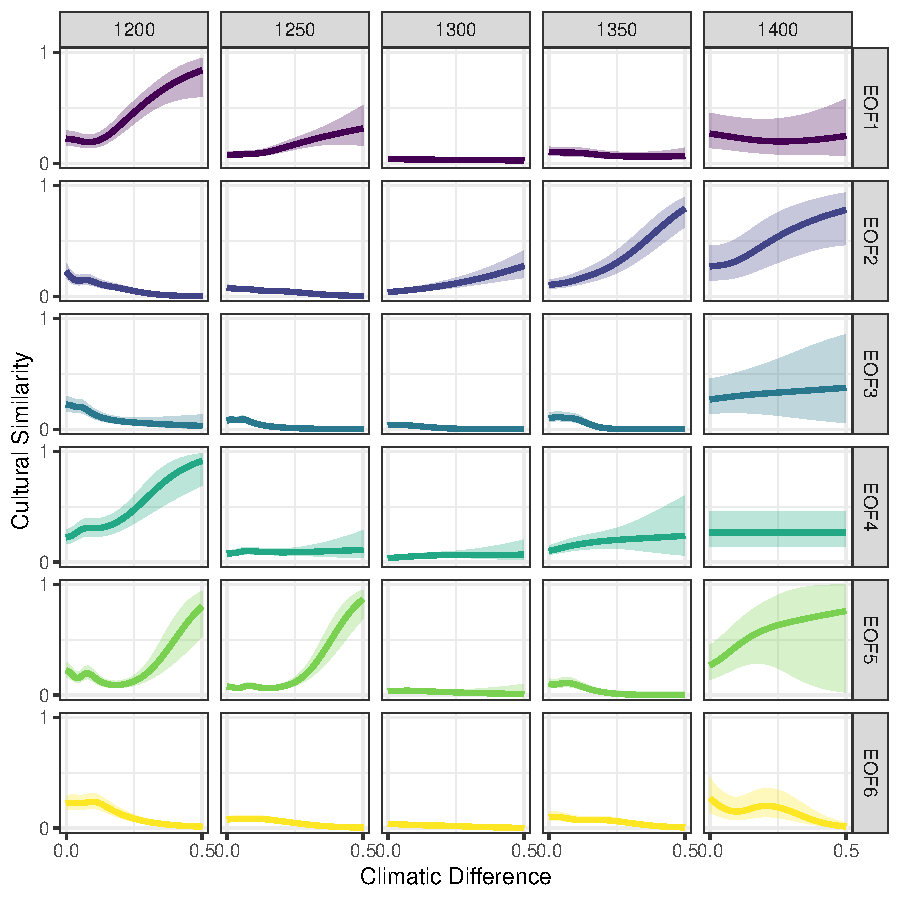
\includegraphics[width=.6\linewidth]{figures/smooths.pdf}
\caption{Estimated smooth functions.}
\label{fig:smooths}
\end{figure}



\subsection*{Much of the variability in social interaction remains unexplained}

\begin{figure}[!htbp]
\centering
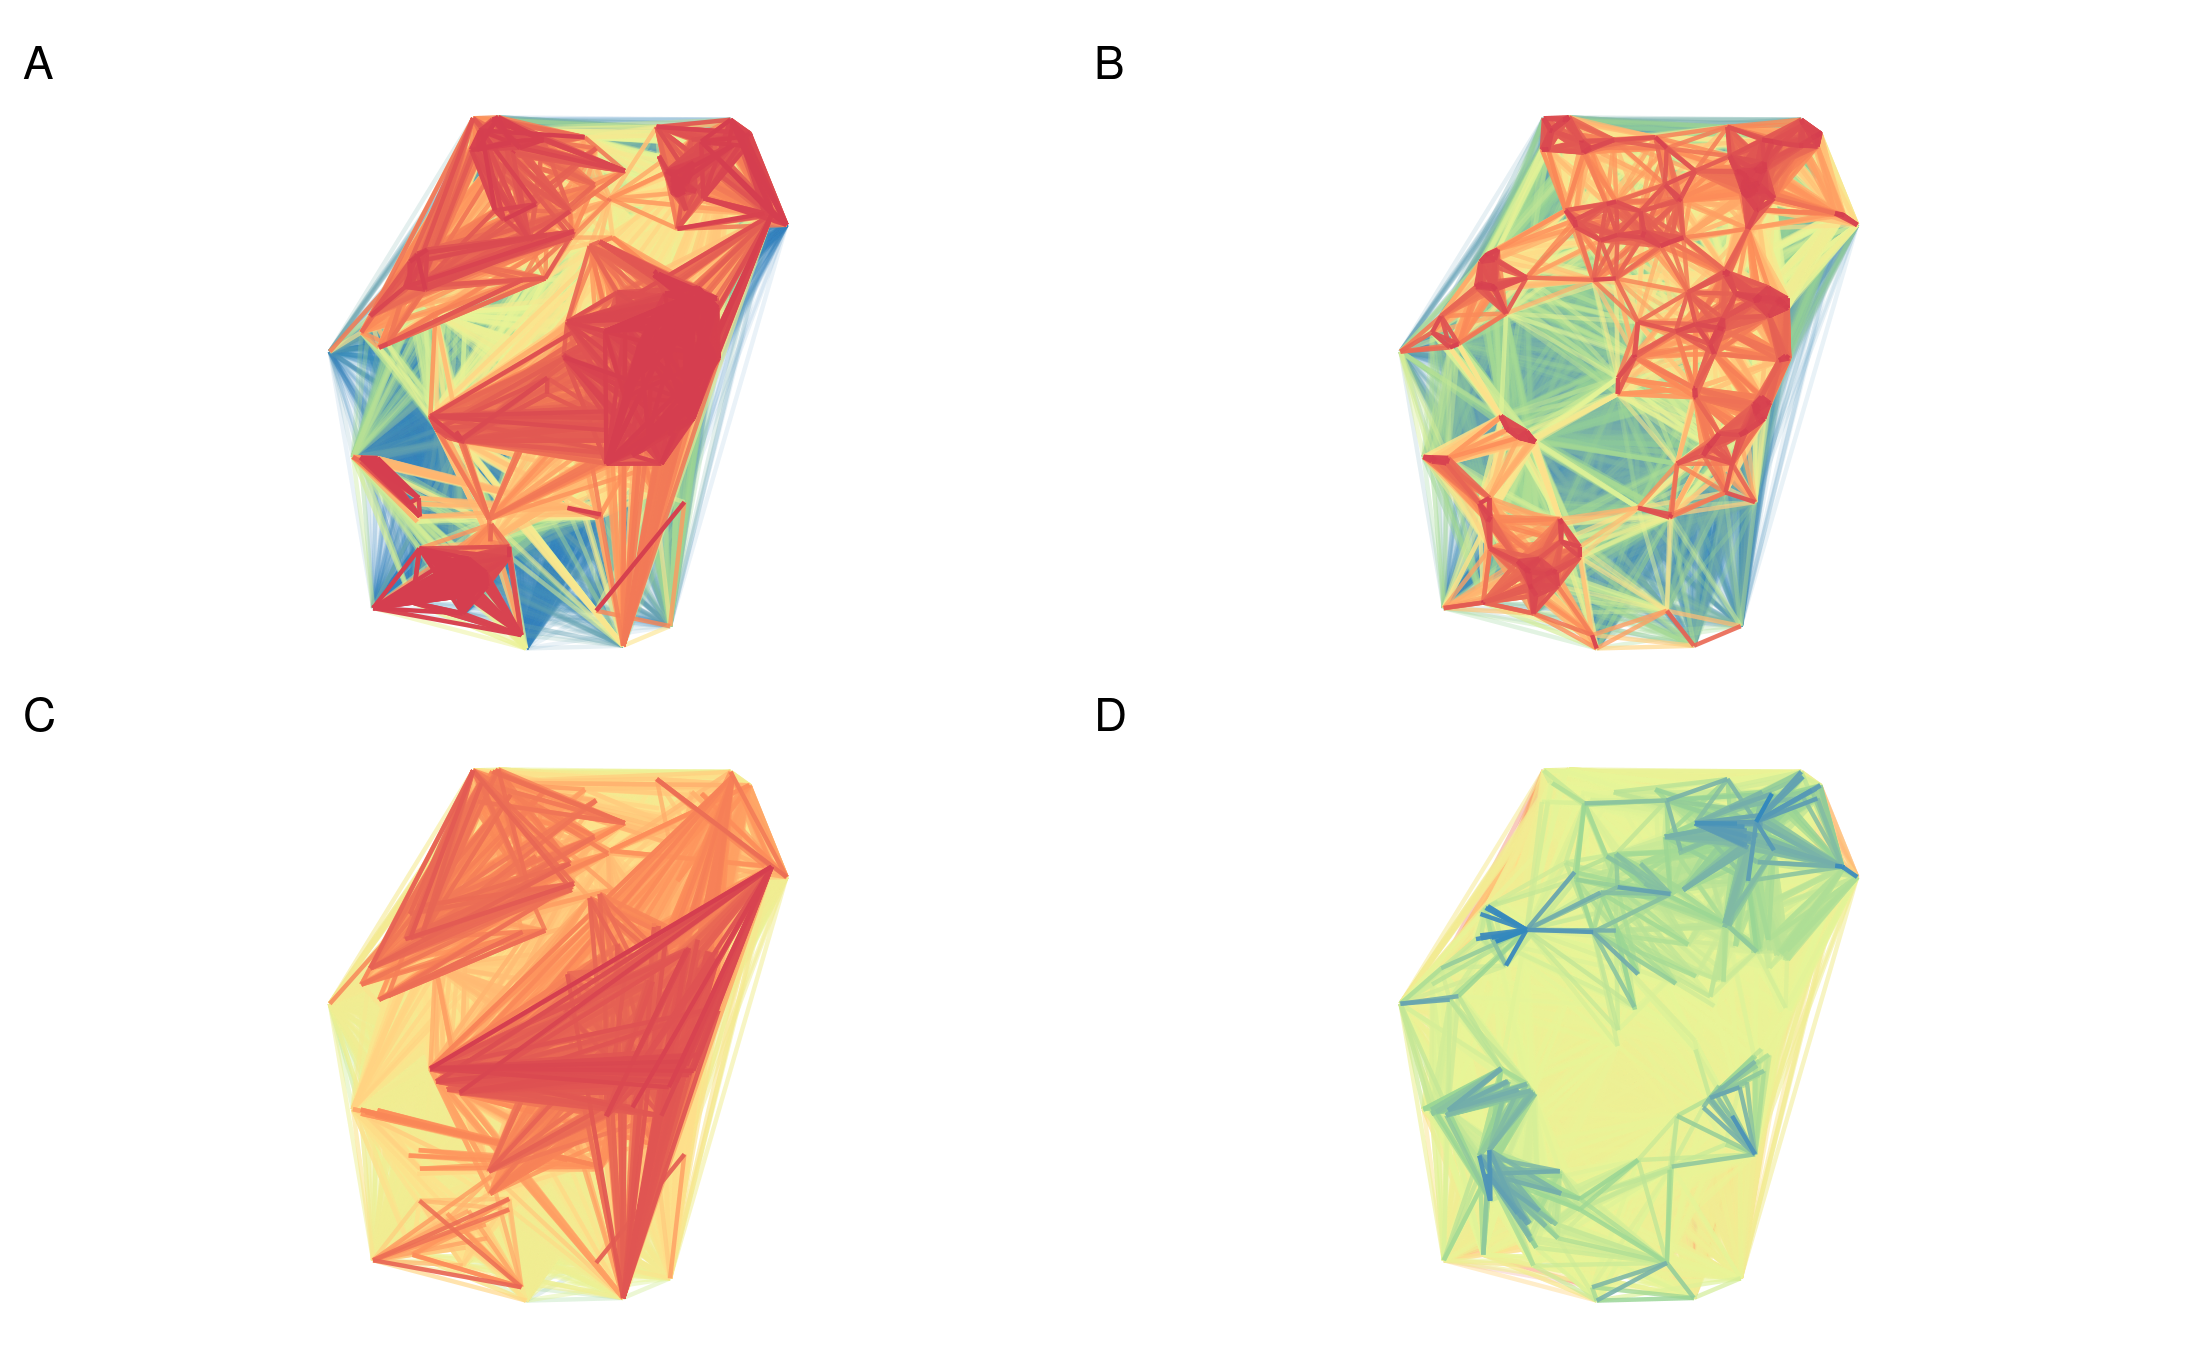
\includegraphics[width=.8\linewidth]{figures/null_model.png}
\caption{A Observed network. B-D are the distance model and the positive and negative residuals, respectively. E-G are the same but for the drought variability model.}
\label{fig:residuals}
\end{figure}

The residuals from the fitted network models still display clear unexplained structure (Figure \ref{fig:residuals}). The distance-only model fitted with the exponential deterrence function predicts a rather sharp falloff in interaction at distance. As expected, the resulting distance-based network predicts many strong interactions at close distances. This is confirmed by the residuals of the model, which show long distance triangular interactions. These broadly correspond to large cultural clusters, a common feature in social networks that is not accounted for by either distance or drought variability. On a micro scale, the residuals display a pattern of high transitivity and triad closure, which is to say there are a great many more closed triangle structures than would be expected by chance. Although this feature is common in human social networks, it is also to be expected from the semi-metric nature of the data, as full transitivity is to be expected in a metric with the triangle equality. The residuals where corresponding to ties that are much less than expected by distance also reveal structure. I see strong directed and spatially discrete clusters of negative interactions that are associated with a pair or few of sites. This may suggest areas of increased conflict, where the kind of social interaction through which pottery would have been exchanged would be rare, or other unmodeled costs of travel such as river crossings cultural taboos. 

%zuni and hopi

%changes in rho value over time -- pointst tomore idiosyncratic interaction

\section*{Discussion and Conclusions}
Rautman (1993 TODO cite) compared the similarity of ceramic assemblages between archaeological sites in central New Mexico to present-day weather station data and found evidence for differential ``investment of social energy in the maintenance of social ties'' between regions with negatively correlated rainfall. Cordell et al. (2007 TODO cite) also compared ceramic assemblages to patterns of rainfall variability, in this case they used 28 tree ring chronologies to to isolate robust patterns of spatial covariability in the four corners region. They found two principal modes of variability reflecting Pacific and Atlantic zones of influence, respectively, and suggest that that broad ceramic regions visible to archaeologists reflect ``maximal risk sharing networks'' that connected communities spanning these zones. Most recently, Strawhacker et al (XXXX todo cite) also used tree ring reconstructions of precipitation to estimate optimal risk sharing networks for archaeological sites in south central New Mexico, but found little evidence that these potential networks corresponded to those in the real world. Johnson finds some evidence for increased marriages between different average climate zones (coastal and inland) but the effect is weak compared to distance and  size. The r2 was .43 for distance and size, and adding dummy variable for same or different environment only increases model to .44.

The specific biophysical contexts of exchange are key, including the temporal dynamics of the entities being exchanged as well as the specific combination of climate mean and variability, and specialized agricultural economies are particular more limited by by interannual deviations than average conditions \cite{Freeman2014}. Sharing and exchange are critical for maintaining population in response to interannual climate variability, although this short term stability can come at the cost of long term environmental degradation \cite{Janssen2010}.
This work says nothing about the role of drought in \textit{producing} similarity, such as a drought leading to many migrants, but rather looks at long term patterns in the costs and benefits of traveling between specific pairs of settlements. This is because I integrate out the mean of each site to get attractiveness, effectively integrating out utility measures (bavaud 2002, 2008). So we are specifically looking at the "deterrence" effect of climate distances, that is the costs and benefits of interaction.
The eof patterns are in part scale dependent. This isn't necessarily a problem, its a necessity that the answer to the question what kind of variability matters is inherently tied to the scale at which on asks the question, there are no right or wrong answers. Although the particular choices of variables, resolution, domain size, truncation level, were informed here by theory and tested to as to minimize sensitivity to particular choices made by the authors, different researchers could still generate equally reasonable results given  different input parameters.  This is simply to state that the drought patterns highlighted here, while I am confident they are not statistical artifacts, should be used with caution in contexts outside of the specific context here.
%The goal here is to extract robust patterns of climate variability. Measures of point-based sample correlation can easily be dominated by noise or other issues with sampling variability. The method we use here yields similar results in appearance, but in a more objective fashion designed specifically to skillfully extract signal from noise.

This study sought specifically to investigate the impact of effective distance and drought variability using statistical models, specifically focused on the functional forms of these relationships. Future study will leverage these findings to construct dynamic simulation models. This will allow us to capture year-to-year variability, as well as the time averaging and bias introduced by archaeological investigation.

Tracing the flows of food, water, and energy within these complex social-ecological systems is essential for understanding their long-term behavior, and leveraging our archaeological understanding of why societies succeed or fail will be critical to anticipating the impact of impending climate changes on farming communities in the developing world.

Importance of the ritual contexts of exchange (Plog 19xx, ford 1972). The eof patterns are the selective enviornment in which norm and institutions regulating social interaction emerge. 

Our data set is not spatially extensive enough to sample the range of hydroclimate variability. For example, the 5th and 6th eofs are not greatly expressed in our study area. But there is evidence for long distance exchange between new mexico and great plains cultures (Speilman 1983) whihc would be consistent with that pattern influenceing exchange. <<(that context is a about nutritional mutualism, not risk reduction).

There remains considerable diversity in the functional response to drought variability. Based on the risk reduction model we would expect negative homophily on drought regime. Yet, the increased differences in drought regime are just as likely to inhibit social interactions as they are to enhance them. This pattern suggests that climate regimes are serving as a deterrent to social interaction in some way, either as ethnolinguistic divisions or conflict. The evidence for conflict and warfare is equivocal (leblance, kobler et al 2016) but largely points to increased resource variability as a source of conflict. So although drought patterns do influence social interaction, the nature of the interaction varies over time and depends on the specific mode of variability. One explanation is that large scale climate regimes influence ethnolinguistic groups. Save for in boundary zones, small scale quotidian interaction would prefer shared ethnolinguistic affiliation. Interregional exchange may occur higher up a sociopolitical hierarchy, as the flows of goods and information proceeded hierarchically. Perhaps then the strongest signal of interaction is between terminal sites, and takes the form of more elite focused ceremonial interactions such as the grain transfers between Mesopotamian god kings.

%points to discuss:
%1. Why doesn't size matter?

%2. Why do things change over time?
%23. These patterns are only what weve seen in the observational record, there could be others
%3. What does ceramic assemblage similarity even mean?
%3b. fully connected widhgted network, but what if pruned?
%  we argue here our approach here is appropriate because we are aggregating many, sparse social networks of individuals together at the population scale. that is we look at macroscale flow patterns given microscale social networks, maxent approach means we make the fest possible assumptions about the configuration of the microscale social networks
%5. Importance of asymmetry. citing crabtree talk about asymmetric debts. also talk about differences in population size and gravity model. what do we miss out on when use symmetric data?
% zuni and hopi? seemingly different because different external vs internal tie patterns, but actually they both cross climate zones
%6. we just looked at summer growing season, but what about winter (where bimodal)? Site coates et al 2015 for variability in the seasonal phasing of rainfall



%The populations of the late pre-Hispanic period in the American Southwest subsisted mainly on maize production, supplemented by a mix of beans and wild proteins. Food transfers are thought to have occurred primarily in the context of informal sharing within kin groups, reciprocal exchange at ritual ceremonies and festivals, and residential mobility on the scale of one to three generations \cite{Hegmon1991,Hegmon1996,Kohler1996TheAnasazi,Varien1999SedentismBeyond,Cordell2007MesaMigration}. The archaeological record attests to extensive exchange networks of durable goods such as ceramics and obsidian \cite{Mills2013a}, and there is direct (if limited) evidence for the long-distance transport of maize \cite{Benson2009PossibleMexico,Benson2010WhoDrought}. There is also evidence for long distance migration (TODO cite mills again?)

%% maybe break these up and cite as exmamples of x method, so reautman for useing BR coefficients and ceramic assemblages as a measure of socialinteraction (that is archaeologically accessible), cordell et all for modes of variability rather than correlations, and strwahacker et al for 


%cordell et al he argue that this pattern breaks doesn ca 1239-1488, and explain it as the source of disruption in this period as the social networks that developed to cross it over the centuries were not able to adapt in time to the temporarily distinct precipitaiton regime. -- this is an important point, and why networks aren't always just optimally minimizing correlation, they take time to build and effort to maintain, especially on the time scales greater than a singel generation. so they are specifically forming in response to robust patterns of variability. In the future it will be important to model the evolution of paths separately, a la bevan and wilson, in order to capture this time lag effect.



%jensen inequality, E(logit(y)) >=logit(E(y)). this means we should interpret specific predictions and confidence intervals from this model with caution, and instead only focus on interpretaiton of the brod functional forms. Its a necessary evil here, becuase we do not yet have the computational abiliy to fit the corMLPE correlation structure and a beta family. Preliminary tests with the data suggested that the pairwise correlation structure was a much alrger source of bias then transforming the response variabble,so that's the tradeoffwe went with. The bias from transforming the respone leads to bias in the estimates of variance





%Social infrastructure interacts directly with physical infrastructure because social networks often must map onto spatial networks. Metabolic costs, such as the energy expended producing and transporting food over space where transportation infrastructure is sparse, provide constraints on energy flows in exchange systems \cite{Drennan1984}. In any particular case, the balance between these costs and the metabolic benefits of social interaction influences whether resources are moved in bulk to populations in need, or whether those populations move themselves to the available resources. The topology of spatial networks also constrains who can interact with whom, introducing bottlenecks and other structural flow constraints \cite{Barthelemy2011SpatialNetworks}. Improvements to transportation infrastructure, such as roads and trails, decrease the effective distance between different settlements; failure to maintain these transportation networks increases the effective distance \cite{McCall1985TheAfrica}.

%Future work should explore more axes of climate variaiton, includeing



%this unconscious discertization is a problem because at the scale of the archaeolgoicaly record we are coarse grianing to coninuous social relaitonships, flows, between human populations, that are teh coarse grained results of small scale interactions, which may themselves be discrete. Individuals may use simple heuristics such as near and far or similar or not, but when a great many of these indivudal discete interactions occur the averaged result is a large scale continuous flow.


\section*{Data and Methods}

\subsection*{Archaeological similarity networks}

The Southwest Social Networks (SWSN) database is a compendium of material-culture data from nearly 1,000 well-dated sites in Arizona and western New Mexico from between 1200 and 1500 CE \cite{Mills2012,Mills2013a,Peeples2013,Borck2015,Hill2015,Mills2015a}. Drawing on a large sample of sites from the earlier Coalescent Communities database of all recorded prehistoric settlements with more than 12 rooms in the Southwest from 1200 to 1700 CE \cite{Hill2004}, the SWSN project analyzed nearly 4.7 million ceramic artifacts and nearly 5,000 obsidian artifacts \cite{Mills2015a}. Using an index of the similarity of ceramic assemblages as a proxy for the intensity of social interaction between settlements, the SWSN database provides quantitative estimates of the topology of the region-wide social network during six 50 year time steps \cite{Mills2013a}.

We start with a symmetric similarity matrix $\mathbf{T}$ with elements $T_{ij} = T_{ji} = BR_{ij}$ with $BR$ defined as the scaled Brainerd-Robinson coefficient of similarity between the proportions of decorated ceramic ware types.

$$BR = 1 - \sum_{k=1}^{p} \lvert P_{ik} - P_{jk} \rvert$$

where $P_{ik}$ is the proportion of ceramics of type $k$ at site $i$.

This metric estimates the similarity in the ceramic discard assemblages between pairs of sites, which in turn is a proxy for cultural preferences, food consumption differences, access to raw materials, and access to trade networks. The index can be loosely interpreted as a probability of interaction between two sites, with identical patterns of ceramic discard indicating a high likelihood of interaction via either direct migration or trade or indirect cultural diffusion.

This is a standard metric in archaeology (cowgill 1990, golitko et al 2009, hart engelbrecht 2012), similar to the xy distances used in other fields.

\subsection*{Spatial interaction model}
Distribution of each person's subjective predictions about the costs and benefits of social interaction, conditional on the information availabile to them about each potential desitmation. Regional sclae patterns of spatial interaciton arise from the decisions of heterogenous agents interacting with impercef and incmpelte information. They make decisions based on the perceived costs and benefits of interation, as far as they can distinguish them. Any cognitive biases held by these agents will impact the aggregate behavior of the system.

Spatial interaction models account for this endogenous structure using entropy maximization techniques, which ensure that simulated networks satisfy simple self-consistency constraints, such as that the sum of outflows of from a region is proportional to its inflows.
I will then use nonlinear regression (generalized additive models for beta-distributed data \cite{Wood2006a}) to determine whether the patterns of interaction strength from the SWSN database are significantly related to the patterns of variability captured in the EOFs.
We fit generalized additive mixed models, and select the most parsimonious model from all candidate models using Akaike's Information Criterion. AIC selection between linear mixed models outperformed several other estimating techniques in landscape genetics in simulation studies by \cite{Shirk et al 2018}. We account for nonindependence of observed edges that share origin or destination sites using the maximum likelihood population effects correlation structure, which models the co dependence of errors on shared sites. This helps account for the nature of pairwise data, including overpowered.


Simple ``gravity'' style spatial interaction models predict the strength of interaction between spatially-distributed populations as a function of their size and distance. Gravity or spatial interaction models are used across the social and natural sciences, but here we use the approach most similar to that in genetics. More generally, a spatial interaction model can predict any flow -- goods, people, and information -- between two entities as a multiplicative function of a set of unkown variables influencing the production and attraction of flows as well as measures of their mutual separation

\begin{equation}
    T_{ij} = v_iw_jc_{ij}
\end{equation}
Spatial interaction models have become popular in archaeology as generative simulation models. Fitting these as stiatistical models to archaeological flows is rare. Here we use the GLM regression approach as commonly used in geograpy, economics, and ecology. Because empirical work on this sale and type is rare we have no exact functional expectations fo the specific terms in (1), so I use Generalized Additive Models (GAMs), a semiparamtric nonlinear regression technique. Specificaly, I fit models of the form

\begin{equation}
    JSD_{ijt} = logit^{-1}\left( f(distance) + f(size) + f(from)_t + f(to)_t\right)
\end{equation}
where f() refers to an arbitrary spline fit using penalization, and from and to are time-varying random effects for the nodes incident on each edge. logt-1 is the inverse logit function, which maps from $(-\inf, \inf)$ to $[0, 1]$. I estimate this equation using restricted maximum likiliohhd and beta regression, wehre we assume JSD is beta distributed with mean $\mu$ and precision $\phi$ estimated during fitting. For robustness, we also estimated this function useing the maximum likelihood population effects correlation structure on the logit transformed data. We compared candidate models using AIC BIC, and R2, and using maximum likelihood, and refit the selected model with REML because of the latter method's better performance.




 
 we aggregate at 10km grid cells so that the results are less sensitive to local settlement dispersal or aggregation.
 %coarse graining data. what if we aggregate at 5km intervals, what about at regional intervals. better estimate of the heirarchy of flows.
 This is because an area of about 10 km radius from a site is the limit of raw material resources for ceramics (TODO cite Arnold1985)
 So 5km is roughly the limit of day to day social interaction, 10km is raw material procurement for ceramics, and 18 km is for day's journey round trip (TODO cite varien). translated to square units in equivalent areas, thats 3km square cells for regular face-to-face interaction and intensitve agriculture. 12km for food and non food resources, and 32km grids for day's trip there and back. so 12 is the most reasonable
 


\begin{equation}
T_{ij} = k v_i^\mu w_j^\alpha \exp(\beta c_{ij})
\end{equation}

where $c_{ij}$ is some notion of the generalized cost of moving from $i$ to $j$ and is symmetric, meaning $c_{ij} = c_{ji}$.Gravity models of this form are quasisymmetric, and can be decomposed into symmetric and asymmetric components. 
Archaeological similarity networks have three features that make traditional spatial interaction modeling difficult. These are 1) the data are bounded between 0 and 1, 2) the measures are symmetric
3) The observations have higher order dependencies.

The network displays a high degree of clustering. This means there are more transitive triads than expected by chance. This is a common feature of social networks (Granovetter XX), friends of friends ar elikely to be friends. This is also something we'd expect a priori in correlation networks (gergm citeation). In our example, if site A is in a differnt drought regime than B and C, we would predict greater interaction from a to those two cites. But given the fact that we are looking at similarities, B and C will appear to be similar from their shared contact with A even if there is 0 contact between them directly. We need to model this dependiencu in the network.

We use this basic principle to fit regression models of the form

\begin{equation}
\begin{split}
    g(E(Y_{ij})) = \alpha + \sum_k f_k(x_k) + \tau_i + \tau_j + \epsilon_{ij}, j = 2, ..., n, i = 1, ..., j - 1\\
    g(x) = log(\frac{x}{1-x})\\
    \tau_i \sim \mathcal{N}(0,\,\sigma^{2}_{\tau})\\
    \epsilon_i \sim \mathcal{N}(0,\,\sigma^{2}_{\epsilon}),
\end{split}
\end{equation}


Which states that the flow of people, goods, or information from site $i$ to site $j$ is a function of some property $v$ of site $i$, property $w$ of site $j$, and the distance between them $c_{ij}$ with $c_{ij} = c_{ji}$

A key question is how to relate directed, asymmetric flows in $T_{ij}$ to the undirected, symmetric similarities in $BR$, that is what is $BR = f(T_{ij},T_{ji})$, which is to say how does ceramic assemblage similarity reflect the underlying flow of people, goods, and information?

\subsection*{Topography and Least-Cost Networks}
The topography of the study area was represented using 90m SRTM DEM, resampled to 250m. A cost matrix was calculated containing, for each DEM cell, the amount of time in seconds it would take a hiker to move to each of the 16 neighboring cells. Time costs were calculated using a version of Tobler's hiking function, which estimates walking speed from terrain slope. The function was modified to make it isotropic (i.e. averaging the uphill and downhill walking speeds) and adding an extra penalty to very steep slopes consistent with human cognitive biases. The walking speed values were then converted into absolute time by dividing each pair of neighboring cells by their inter cell distances. This cost matrix (time) was then inverted to represent conductances (speed), facilitating a sparse matrix representation and estimation fo least cost paths using efficient graph theoretic algorithms in gdistance. The resulting transition matrix was used to calculate all parisiw isotropic least cost paths between each pair of archaeological sites.
% This full pairwise distance matrix likely underestimates the effectivedistance between archaeological sites, as travellers would have been likely to prefer passng through intermediate settlements rather than making a single long direct journey. Especially on long distance dripts through resource poor environments. So for each time step, the full distance matrix was pruned to a 10 nearest neighbor network in each time step. Pairwise travel costs for all successive analyses were then calculated using the k shortest paths along this pruned network, rather than useing the full pairwise least cost paths.

%We focus on the perceived time costs of travel. In rugged, mountainous terrain, slope is the key factor in influencing ease of travel. We focus specifically on paths, or the pysical routes that people trtaveled. A good path connects ing two places has to ptimize for ease of travel in both directions. People will consistently overestimate slopes, so the perveived cognitive costs of moving across the landscape will be greatr. So we are focusing on these mental paths, as long as they influece who people choose interact with. Paths are physiucal and social infrastructure.

All else being equal, locations that are closer together in space will be more similar than those further apart \cite{Tobler1970}. Modelling this spatial structure in the SWSN data is necessary to control for spatial dependence in statistical analyses of these data. To accomplish this, I calculate the least-cost network between all sites in the SWSN network. This method provides an efficient estimation of the metabolic costs of movement between any pair of settlements in the network. I calculate these costs using the Pandolf-Santee formula \cite{White2012}, which relates the metabolic rate of a traveler in watts to the traveler's weight and external load, walking speed, terrain slope, and a dimensionless terrain roughness coefficient. Using energy expenditure rather than time or Euclidean distance to represent movement costs facilitates a direct comparison of the metabolic costs and benefits of food transfers  \cite{Drennan1984}. The resulting least-cost network will be used as a proxy measure for the constraints on moving both people and bulk goods across the landscape, and thus the topographic affordances for social exchange.



\subsection*{Modes of hydroclimate variability}
To isolate meaningful patterns of variability in the paleo-reanalysis, I use the model outputs to calculate a drought index and then decompose the nearly 3,600 monthly drought maps from 1200 to 1500 CE into five \textit{empirical orthogonal functions} (EOFs). EOFs are the eigenvectors of the climate space-time covariance matrix, such that the leading EOFs capture most of the variability in the original climate signal \cite{Lorenz1956EmpiricalPrediction}. EOFs are equivalent to the principal component analysis commonly used in archaeology \cite[e.g.]{Dean1996DemographyStress}, save for that the principal components of a spatiotemporal dataset only capture temporal signals.

varimax rotation, scaled by the square root of the corresponding eigenvalues
retained modes based on variance explained, degree of separation of the eigenvalues, Norht's rule of thumb, scree test. We controlled for temproal autocorrelatio in the data by estimateing the efective sample size, and generated confidence intevalas for the eigenvalues as a result.

\subsection*{Drought reconstruction}
As a measure of drought variability, I analyzed the 100 year dataset of 12 month SPEI calcualted from PRISM data. First I calculated the empirical orthogonal functions via a singular value decompsoition of the space time covariance matrix. This step is equivalent to working on the correlation matrix, as SPEI is already standardized to unit variance at each location . I multiplied each cell by the cosine of latidued to account for areal distortion effects. I then selected the leading eigenvalues for rotation, using a combination of scree test and North's rule of thumb, which accounts for autocorrelation in the ovserved data. I then rotate dthe elading eigenvalues using a varimax rotation in order to rlea the spatial orhtogonality constraints of the EOF ansalysis and to reveal coherent, physically meaningful patterns. The resulting eigenvectors were then multiplied by the square root of the corresponding eigenvalues to yield correlation coefficients. The REOF amplirdut time serise was then compared to the observational record, and the signs fo the eigenvalues and vectors were reversed to match the histoical record (so that a positive time series value corresponds to a positive spei and vice eeras).

In order to confrim these patterns, the REOS were compared to those claculated from a 1,000 year reocnstuction, from which the associated patterns were also extracted.


ccsm simulates monsoon ok, better than others. 
Its able to represent eogs and teleconnections (seager and hoerling 2014, that other paper)

For the late pre-Hispanic period of interest, I will use outputs from the Community Earth System Model (CESM) Last Millennium Ensemble (LME) as a model prior. LME is a paleoclimate simulation that uses CESM to recreate the transient response of the global climate system to changes in climate forcings (e.g. orbit, greenhouse gasses, volcanic activity, land-cover change) during the past 1,000 years \cite{Otto-bliesner2015}. Data assimilation techniques such as the ensemble Kalman filter are used to generate atmospheric \textit{reanalyses}. A reanalysis is a model-based climate hindcast optimally constrained by instrumental observations. Paleoclimate data assimilation relies on the same principle but replaces instrumental observations with paleoclimate proxy records such as tree rings, ice cores, and corals \cite{Hakim2016TheResults}. Paleoclimate model simulations serve as physically consistent prior information about the possible states of the climate system, and the proxy records provide novel information about the time evolution of those states. The ensemble Kalman filter uses this information, as well as the spatial covariances from the climate-model prior (e.g. teleconnections), to "spread out" information from the point-based proxies to generate physically optimal extrapolations beyond the proxy locations \cite{Acevedo2015TowardsTechniques,Hakim2016TheResults}.





\bibliography{references}


\section*{Acknowledgements (not compulsory)}

Acknowledgements should be brief, and should not include thanks to anonymous referees and editors, or effusive comments. Grant or contribution numbers may be acknowledged.

%\section*{Author contributions statement}

%Must include all authors, identified by initials, for example:
%A.A. conceived the experiment(s),  A.A. and B.A. conducted the experiment(s), C.A. and D.A. analyzed the results.  All authors reviewed the manuscript. 

\section*{Additional information}

To include, in this order: \textbf{Accession codes} (where applicable); \textbf{Competing interests} (mandatory statement). 

\end{document}